In this section we first motivate our microservice approach based on our
experiences developing the MIxT web application. We describe the process from
initial data analysis to the final application, highlighting the importance of
language-agnostic services to facilitate the use of different tools in different
parts of the application. We show that these services are easy to deploy and
provide performance to use them to build data exploration applications.
We then generalize the ideas to a set of principles and services that can be
reused and shared between applications, and show their design and
implementation. 

\subsection*{Motivating Example} 
The aim of the Matched Interactions Across Tissues (MIxT) study was to identify
genes and pathways in the primary breast tumor that are tightly linked to genes
and pathways in the patient blood cells.\cite{vanessa} We generated and analyzed expression
profiles from blood and matched tumor cells in 173 breast cancer patients
included in the Norwegian Women and Cancer (NOWAC) study.
The MIxT analysis starts by identifying sets of genes tightly co-expressed
across all patients in each tissue. Each group of genes or modules were
annotated based on known a priori biological knowledge about gene functionality.
Focus was placed on the relationships between tissues by asking if specific
biologies in one tissue are linked with (possibly distinct) biologies in the
second tissue, and this within different subgroup of patients (i.e. subtypes of
breast cancer).

We built an R package\footnote{\url{github.com/vdumeaux/mixtR}} with the
statistical methods and static visualizations for identifying associations
between modules across tissues. The exploration of the results encompass the
examination  of $\sim20$ modules and their functional enrichments. That is
$\sim23\times19=437$ associations computed for each of the $22$ patient
subgroups. 

To explore this large amount of data and results we needed an interactive
point-and-click application that could interface with the statistical methods
and link the results to online databases. This would make it possible for users
to explore the results without any coding background. We needed an application
that could interface with MSigDB to fetch gene set meta-data and the Entrez
Programming Utilities (E-utils) to retrieve gene meta-data. To make the
interfaces to the statistical analyses and databases re-usable by other
applications that we aim to implement later it was necessary for these to
communicate using open protocols. 

In addition, we required that the application was containerized. This allows us
to deploy the application on a wide range of hardware, from local installations
to deployments to cloud providers such as Amazon Web Services
(AWS)\footnote{\url{aws.amazon.com}}. 

\subsection*{Design}
Our experience can be generalized into the following design principles for
building applications in bioinformatics: 


\textbf{Principle 1}: Build applications as collections of language-agnostic
microservices. This enables re-use of components and does not enforce any
specific programming language on the user-facing logic or the underlying
components of the application. Within bioinformatics, researchers and
application developers use a wide range of programming languages to build tools.
By composing an application of services communicating over standard protocols it
is possible to re-use existing tools in new applications. 

\textbf{Principle 2}: Use software containers to package each service. This has
a number of benefits; it simplifies deployment, ensures that dependencies and
libraries are installed, and it simplifies sharing of services between
developers. 

Using these design principles we built the MIxT web application using the
microservices in Kvik to interface with statistical analyses and biological
databases. Kvik provides a compute service for executing statistical analyses and a
database service for retrieving relevant information on genes and biological
processes.  Using these it is possible to develop specialized data exploration
application in any modern programming language.  In the rest of the section we
discuss the design choices we made to build the microservices that power the
MIxT web application. 


\subsubsection*{Compute Service}

The main cornerstone of every data exploration application in systems biology is
a dataset. Datasets go through a series of transformations before they can be
interpreted by experts. Because of the complexity of these datasets, package
repositories such as BioConductor provide software for reading and analyzing the
data. Because of the complex datasets, there are a number of requirements for
systems that can explore them
i) datasets require specialized software to be read,
ii) datasets can be too big to fit on a desktop computer,
iii) statistical methods for analyzing the datasets are too computationally
intensive to run on a desktop computer, 
iv) users may want to modify statistical analyses directly from an application, 
and 
v) users need to know exactly what transformations has been done to a dataset to
reproduce the analyses. 

From these requirements we have designed the compute service in Kvik. The compute
service interfaces directly with the R programming language, making it possible
to call functions from any R package. Application developers can use the
compute service to execute analyses and return results. By interfacing directly
with R developers can leverage this to produce dynamic applications. For example,
if an application uses a clustering method to color nodes in a graph, end-users
can tweak parameters that interactively within the application that changes the
node coloring in graph visualization. Also, by interfacing with R directly from
an application it can store provenance data on the statistical methods and input
parameters being used. 
By placing data storage and analysis into a service, application developers can
deploy it on a powerful server while keeping the user-facing application logic
on the desktop. Packaging the service into a software container also
provides the necessary functionality to ensure that the statistical analyses can
be reproduced later. 

The compute service offers three main operations to interface with R. 
i) to call a function from an R package,
ii) to get the results from a previous function call,
and iii) a catch-all term that both calls a function and returns the results. 
We use the same terminology as OpenCPU\cite{opencpu} and have named the three
operations Call, Get, and RPC respectively. These three operations provide the
necessary interface for applications to include data in the applications.

\subsubsection*{Database Service} 
To understand analysis results experts query databases and scientific
literature. There are a wealth of online databases, some of which provide open
APIs in addition to web user interfaces that application developers can make use
of. While the databases can provide helpful information, there are some
challenges including them in interactive data exploration applications: 

i) the APIs aren't fast enough to use in interactive applications where the
application has to perform multiple database calls, 
ii) some databases put restrictions on the number of database calls, and 
iii) there is no uniform way for storing database lookup provenance to reproduce
the database lookups. 

To solve these problems we built a database service for application developers
to include. The service includes a simple caching mechanism that solves the two
challenges. If we cache queries to the database we can speed up subsequent calls
and reduce the load on the respective databases. Both the query from the
application and the response from the databases are stored for later use.
The database service provides an open HTTP interface to biological databases for
retrieving meta-data on genes and processes. We have currently packages for
interfacing with E-utilities\footnote{\url{eutils.ncbi.nlm.nih.gov}},
MSigDB\footnote{\url{software.broadinstitute.org/gsea/msigdb}}, Hugo Gene
Nomenclature Committe (HGNC)\footnote{\url{genenames.org}}, and Kyoto
Encyclopedia of Genes and Genomes (KEGG)\footnote{\url{kegg.jp}}. 


\subsubsection*{Applications} 
Kvik provides services to perform database lookup and execute statistical
analyses. Since we provide both services as software containers, application
developers simply run these and write applications that interface with them.
Using our services application developers have a platform for running
statistical analyses, and a fast clean interface to get metadata about genes and
processes. 

Figure \ref{kvik-mixt} shows how the the MIxT application is built using Kvik
microservices. In MIxT we built a specialized web application that interfaces
with Kvik to get data from biological databases and to run statistical analyses
from the mixt R package\footnote{\url{github.com/vdumeaux/mixtR}}. 

\begin{figure}[h!]
\centering
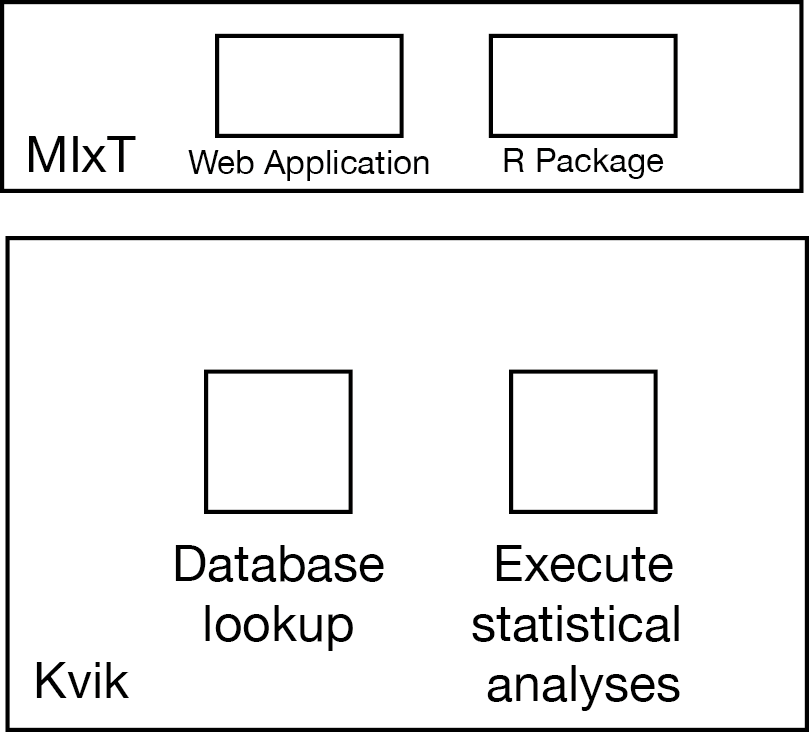
\includegraphics{figures/kvik-mixt.png}
\caption{An overview of the relationship between the MIxT application and Kvik.
MIxT contains a web application (online at \url{mixt-blood-tumor.bci.mcgill.ca})
and the R Package that provides analyses and data to the web application. Kvik
provides the services for running the statistical analyses from the R package,
and the database lookups found in the web application.} \label{kvik-mixt}
\end{figure} 

\subsection*{Implementation} 
In ths section we describe the implementation details of the microservices we
provide in Kvik.

Kvik is implemented as a collection of Go packages required to build services
that can integrate statistical software in a data exploration and provide an
interface to up-to-date biological databases. We chose the Go programming
language because of its performance, ease of development, and simple deployment.
To integrate R we provide two packages \emph{gopencpu} and \emph{r}, that
interface with OpenCPU and Kvik R servers respectively. To interface with
biological databases we provide the packages \emph{eutils}, \emph{gsea},
\emph{genenames}, and \emph{kegg} that interface with E-utils, MsigDB, HGNC and
KEGG respectively.  In addition to these packages we provide Docker images that
implement the two required microservices. 

Both the compute and the databases service in Kvik builds on the standard
\emph{http} package in Go. The database service use the
\emph{gocache}\footnote{\url{github.com/fjukstad/gocache}} package to cache any
query to an online database. In addition we deploy each service as Docker
containers.\footnote{Available at \url{hub.docker.com/r/fjukstad/kvik-r} and
\url{hub.docker.com/r/fjukstad/db}}

\subsubsection*{Compute Service} 
The compute service is an HTTP server that communicates with a pre-set number of
R processes to execute statistical analyses. On start of the compute service
launches a user-defined number of R worker sessions for executing analyses,
default is 5. The compute service uses a round-robin scheduling scheme to
distribute incoming requests to the workers. We provide a simple FIFO queue for
queuing of requests. The compute service also provides the opportunity for users
to cache analysis results to speed up subsequent calls.

The compute service in Kvik is built using a hybrid state pattern.
A hybrid state pattern origins from functional programming, where output from a
method only depends on its inputs and not the program state.\cite{opencpu}. In
practice this means that the compute services stores the output results from
function calls, but can compute them if the service has to restart. This makes
it possible for us to scale the compute service horizontally to handle more
requests. If an R worker session for some reason crashes the compute service
simply starts up a replacement. 

